\documentclass{article}

\usepackage[paper=letterpaper,margin=2.5cm]{geometry} % Set Margins

%% Math and math fonts
\usepackage{amsmath, amsthm, amssymb, amsfonts}
\usepackage{bbm} % for \mathbbm{1}

% date
\usepackage[nodayofweek]{datetime}

% Color
\usepackage{color, xcolor}

% Misc
\usepackage{environ}  % \collect@body in asmmath
\usepackage{graphicx} % \includegraphics options
\usepackage{mdframed} % text boxes
\usepackage{indentfirst} % Indent first paragraph after section header
\usepackage[shortlabels]{enumitem} % Control enumerate items with [(a)]
\usepackage{comment} % Comments
\usepackage{fancyhdr} % Headers and footers

% Tables
\usepackage{array}

% Sub-figures and figure placement
\usepackage{caption}
\usepackage{subcaption}
\usepackage{float} 

% Graphing
\usepackage{pgfplots}
\pgfplotsset{compat=1.17}
\usepackage{tikz}

% Title Placement
\usepackage{titling}
\setlength{\droptitle}{-6em}

%set indent to 
\setlength{\parindent}{0pt}

% Hyper refs
\usepackage{hyperref}
\hypersetup{
    colorlinks=true,
    linkcolor=blue,
    urlcolor  = blue,
    filecolor=magenta,      
    urlcolor=blue,
    citecolor = blue,
    anchorcolor = blue
}

% % Citation management
\usepackage{natbib}
\bibliographystyle{abbrvnat}
\setcitestyle{authordate,open={(},close={)}}

\pagestyle{fancy}

\usepackage[paper=letterpaper,margin=2.5cm]{geometry} % Set Margins

%% Math and math fonts
\usepackage{amsmath, amsthm, amssymb, amsfonts}
\usepackage{bbm} % for \mathbbm{1}

% date
\usepackage[nodayofweek]{datetime}

% Color
\usepackage{color, xcolor}

% Misc
\usepackage{environ}  % \collect@body in asmmath
\usepackage{graphicx} % \includegraphics options
\usepackage{mdframed} % text boxes
\usepackage{indentfirst} % Indent first paragraph after section header
\usepackage[shortlabels]{enumitem} % Control enumerate items with [(a)]
\usepackage{comment} % Comments
\usepackage{fancyhdr} % Headers and footers

% Tables
\usepackage{array}

% Sub-figures and figure placement
\usepackage{caption}
\usepackage{subcaption}
\usepackage{float} 

% Graphing
\usepackage{pgfplots}
\pgfplotsset{compat=1.17}
\usepackage{tikz}

% Title Placement
\usepackage{titling}
\setlength{\droptitle}{-6em}

%set indent to 
\setlength{\parindent}{0pt}

% Hyper refs
\usepackage{hyperref}
\hypersetup{
    colorlinks=true,
    linkcolor=blue,
    urlcolor  = blue,
    filecolor=magenta,      
    urlcolor=blue,
    citecolor = blue,
    anchorcolor = blue
}

% % Citation management
\usepackage{natbib}
\bibliographystyle{abbrvnat}
\setcitestyle{authordate,open={(},close={)}}

% ----------------------------------------
% TITLE
% ----------------------------------------

\pagestyle{fancy}

\lhead{Creel}
\chead{Week Five}
\rhead{AMES}

\title{AMES Class Notes -- Week Five, Day 1}
\author{Andie Creel}

\begin{document}
\maketitle

\section{Review from last week}

\subsection{Notation:}
\begin{align}
    \frac{dF(x)}{dx} = F'(x) \\
\end{align}

\subsection{Chain rule: } Consider $F(G(X))$
\begin{align}
    \frac{dF}{dx} = \frac{dF}{dG} \frac{dG}{dx}
\end{align}

\subsection{We can work with derivatives like fractions.} Therefore, 
\begin{align}
    \frac{dF(x)}{dx} = F'(x) \implies dF(x) = F'(x) dx
\end{align}
This means we went from a \textit{derivative} to a \textit{differential}. This is an important part of notation with integrals as well. The thing to know and remember is that $dx$ just means "small changes." We can divide by small changes (like in derivatives) or multiply by small changes (like in differentials). \\

\subsection{Derivative rule for exponential function, $e^x$}:
\begin{align}
    \frac{de^x}{dx} = e^x
\end{align}
We have proportional change. This is the only function in the world where the rate of change at a point is equal to the function at that point. \\

\subsection{Example:}
Consider the function \[f(x) = e^{ax}\]

We know \[\frac{de^x}{dx} = e^x.\] 

Let's do a u-substitution to make this simpler. Let \[U(x) = ax.\]  

Our function is now written as \[f(x) = e^U.\] 

Recall the chain rule:

\begin{align}
   \frac{dF(x)}{dx} = \frac{dF(x)}{dU(x)}\frac{dU(x)}{dx} 
\end{align}

We want to know what $\frac{dF(x)}{dx}$ is. We can solve for the two simpler derivatives on the right hand side to gt this. 

\[\frac{dF(x)}{dU(x)} = e^U \]
\[\frac{dU(x)}{dx}  = a \implies\]
\[\frac{dF(x)}{dx} = a e^U \]
Now, plug our U-substitution back in: 
\[\frac{dF(x)}{dx} = a e^{ax} \]

\subsection{Example}
Let 
\begin{align}
    F(x) = ln(e^x)
\end{align}
We're interested in the derivative. 
\begin{align}
    \frac{dF(x)}{dx} = 1
\end{align}
Why!? Chain rule, log rule, exponential rule. First, do a u-substitution and apply the chain rule
\begin{align}
    U(x) &= e^x \implies\\
    F(x) &= ln(U(x)) \implies \\
    \frac{dF(x)}{dx} &= \frac{dF(U(x))}{dx} = \frac{dF(x)}{dU(x)}\frac{dU(x)}{dx}
\end{align}
Find $\frac{dF(x)}{dU(x)}$ using log rules 
\begin{align}
    \frac{dF(x)}{dU(x)} = \frac{1}{U(x)}
\end{align}

Find $\frac{dU(x)}{dx}$ using exponential rules 
\begin{align}
    \frac{dU(x)}{dx} = e^x
\end{align}

Now we can plug these results back into equation 11, 
\begin{align}
    \frac{dF(x)}{dx} &= \frac{1}{U(x)} e^x
\end{align}
Plug our u-substitution back in, 
\begin{align}
    &= \frac{1}{e^x} e^x \\
    &= 1
\end{align}

\section{Maximum and minimum}
If you're out hiking, how do you know if you're at the top of a hill? You will walk on flats at the top. We often want to know the peaks and valleys of slopes. When are we at the top? When are we at the bottom? \\

In applied setting we often times want to know when we can maximize and objective or minimize an objective? How much time does a critter spend vigilant to maximize it's chance of survival? How much money should a business invest in climate mitigation strategies to maximize their profit? \\

These questions are interesting on their own. These are the questions that motivate \textit{why} we need to learn calculus, because these questions can be answered \textit{using} calculus. Calculus isn't important on its own, it's important because it can help us answer important questions. 

\subsection{How do we know if we're going to a peak or a valley?}
We can use calculus to find a peak or find a valley. Consider a mountain range that can be modeled with the equation
\begin{align}
    Y = F(x) = ax - bx^2 \\
    a > 0 \text{ and } b > 0
\end{align}
where is a peak/valley of this mountain range? At what level of $x$ is $F(x)$ maximized or minimized?

\begin{align}
    \frac{dF(x)}{dx} &= a - 2bx = 0 \implies \\
    x &= \frac{a}{2b}
\end{align}

How do we know if this is a maximum or minimum (peak or valley)? We can use the \textbf{second derivative}. If the second derivative is negative, it's a maximum. If the second derivative is positive, it's a minimum. (Use Eli's tricks of smiley faces and frowny faces to remember this. If the second derivative is negative, the function is a frowny. If the second derivative is positive, the function is a smiley). \\

A function is concave is the second derivative is negative. A function is convex if the second derivative is positive.\\

\begin{align}
    \frac{d^2F(x)}{dx^2} = -2b.
\end{align}
Assuming $b>0$ implies $-2b<0$ therefore we have a local maximum. \\

Physicists do a good job keeping of functions, first derivatives and second derivatives. It's (respectively) location, speed, acceleration, jerk ("if someone's being really mean to you you can say you're being a really big third derivative" - Eli). 

\section{How the eqn for mean was derived}

\begin{figure}[htp]
    \centering
    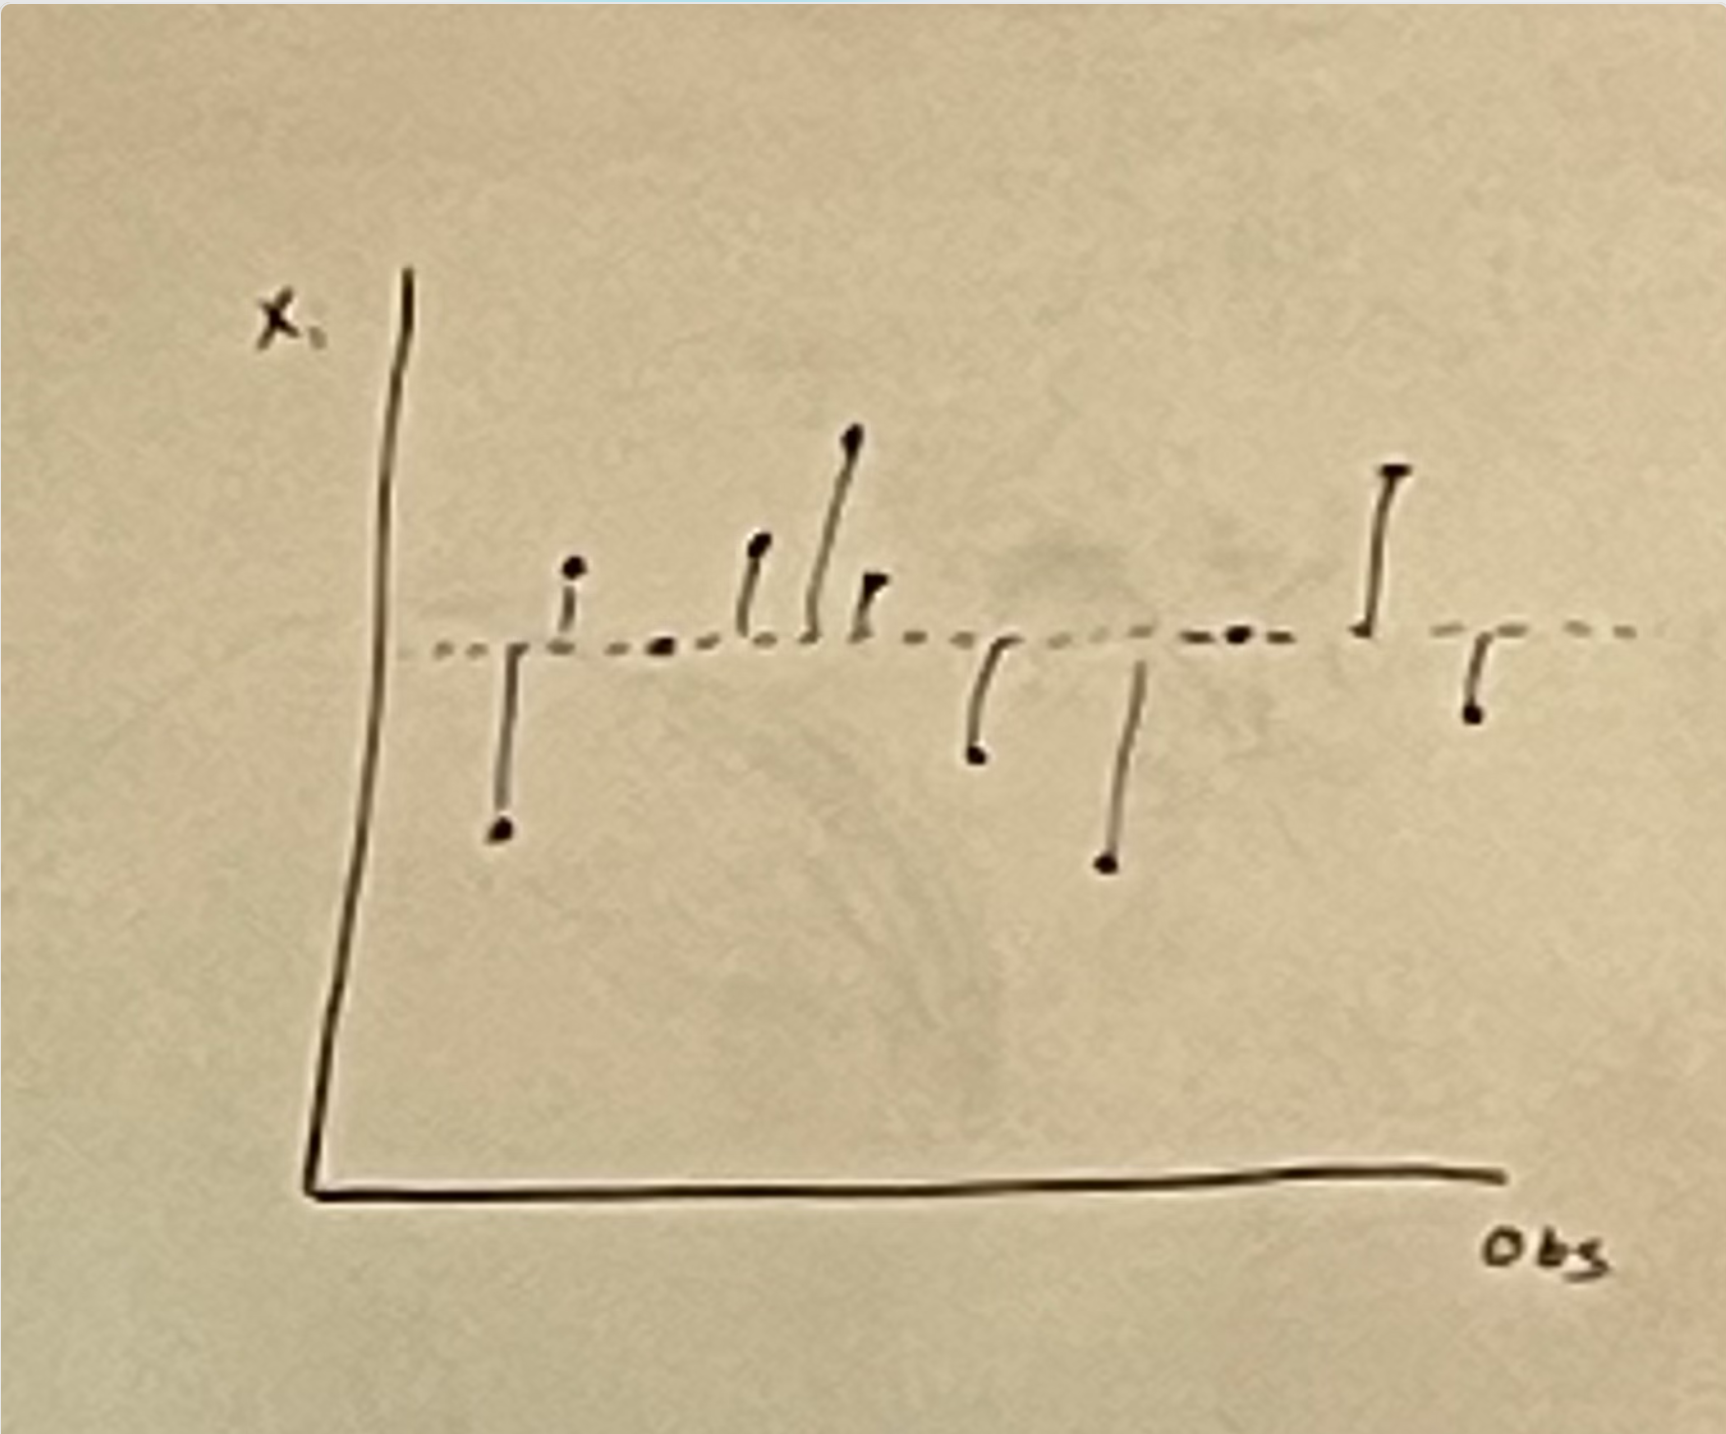
\includegraphics[width=8cm]{mean_pic.png}
    \caption{Dotted line is mean}
\end{figure}

How do we find an average? We want to find an $\bar x$ that minimizes the total distance from $\bar x$, squared. Why are we squaring it? We don't care if $x_i$ is greater that $\bar x$ or less than $\bar x$. We just want to find an $\bar x$ where all $x_i$ are not that far away from $\bar x$. \\

We can define the mean as the $x$ that minimizes the differences between itself and all other $x_i$ observations,

\begin{align} 
    \bar x = \textbf{argmin} \sum_i^N (x_i - \bar x) ^2
\end{align}
Great, we have an equation defining the mean. However, this is not very easy to compute (how do you use an argmin??). It's defined clearly, but we can't calculate it easily. \\


\subsection{Deriving eqn for mean}
Consider the function 
\begin{align}
    F(\bar x) &= \sum_i^N (x_i - \bar x)^2\\
    &= (x_1 - \bar x)^2 + (x_2 - \bar x)^2  + (x_3 - \bar x)^2 +... + (x_N - \bar x)^2
\end{align}

\textbf{Objective:} Find the $\bar x$ that minimizes the distance from itself and all other $x_i$, where the distance between two points $x,y$ is measured as $(x -y)^2$. \\

If we're wanting to \textit{minimize} (getting back to the argmin) the distance from $x_i$ to $\bar x$, we can take a derivative and set it equal to zero: 
\begin{align}
    \frac{d F(\bar x)}{d\bar x} &= -2(x_1 - \bar x)  -2(x_2 - \bar x) -2(x_3 - \bar x) - ... -2(x_N - \bar x) = 0\\
\end{align}
Divide both sides by $-2$, then group the $\bar x$ into one term, 
\begin{align}
    x_1 + x_2 + x_3 + ... x_n - N \bar x &= 0\\
    x_1 + x_2 + x_3 + ... x_n &= N \bar x
\end{align}
plug in summation notation 
\begin{align}
    \sum_i^N x_i = N \bar x \implies \\
    \bar x = \frac{1}{N}\sum_i^N x_i
\end{align}

This is how the \textbf{arithmetic mean} was derived. When someone wanted to find an $\bar x$ that was not that different from all the other $x_i$, they solved this problem! \\

To confirm that $\bar x$ \textit{minimizes} the distances between all $x_i$ and itself, you can take a second derivative and confirm that the second derivative is positive, which means the function is convex and we've found the minimum of that convex function.  

\subsection{Problem set hint}
The hardest problem on the problem set is asking us to derive the process for linear regression. \\

Linear regression finds a conditional mean \textit{aka} a mean conditioned on $x$, which is just a line. \\

In the problem set, we will want to minimize the distance between $y_i$ and $F(x_i)$,
\begin{align}
    \text{distance}=(y_i - F(x_i))^2.
\end{align}
What's $F(x)$ going to be? The previously mentioned conditional mean, \textit{i.e.,} a line. In the problem set, we parameterize a line that minimizes the distance between the data points and the line. Solving this problem solves for the same algorithms that computers use when they fit linear regressions. 

\section{Mean Value Theorem}
\textbf{Definition of Mean Value Theorem}: For a smooth and continuous function, there is at least one point on a given interval where the derivative is equal to the average rate of change over the interval. \\

\textbf{Intuition:} The theorem says that if you draw the secant line (the straight line) connecting the point $(a, f(a))$ (where $a$ is on the x-axis and $f(x)$ is on the y-axis) and the point $(b, f(b))$, then somewhere in the interval $(a,b)$ there will be a point $c$ where the tangent line (the line that touches the curve at exactly one point and has the same slope as the curve at that point) is parallel to the secant line. In other words, at some point in the interval, the function's derivative matches the average rate of change over the interval, 
\begin{align}
    f'(c) = \frac{f(b) - f(a)}{b - a}.
\end{align}

\section{Taylor Series}

We know that straight lines are good approximators because a line is a conditional mean, and means are good at minimizing error.\\

Series are good approximators of sequences of numbers, because series are functions. \\

A \textbf{Taylor Series} is an extremely useful series for approximating the relationship of sequence of numbers (data is a sequence of numbers). Taylor series underpins a lot of the math we do today, particularly for any relationship that isn't linear. 

\begin{align}
    f(x) = f(a) + \frac{f'(a)}{1!}(x-a)^1 + \frac{f''(a)}{2!}(x-a)^2 + \frac{f'''(a)}{3!}(x-a)^3 + ... + \frac{f^k(a)}{k!}(x-a)^k + R
\end{align}
where $R$ is the residual, or higher order terms.\\


\subsection{0th order Taylor Series}
Consider a 0th order taylor series: it would be a \textbf{mean} aka just a flat line equal to $f(a)$. \\

If you're only looking at the means of a dataset, that means you're doing a 0th order taylor approximation.

\subsection{First order Taylor Series}

Consider a first order taylor series: 
\begin{align}
    f(x) &= f(a) + \frac{f'(a)}{1!}(x-a)^1 \\
    &= A + B (x-a) \\
    &= A -aB + Bx\\
    &= m + Bx
\end{align}
It's a \textbf{line} with a slope. A first order Taylor series is a linear approximation. Linear regression is a first order Taylor approximation. \\




% \section{Partial derivatives}
% Consider a function that maps from $R^2 \to R^1$, 
% \begin{align}
%     Z = F(x, y).
% \end{align}

% Consider a situation where we can change $x$ with policy, but we can't change $y$ and we want to maximize outcome $Z.$ In this case, we would take the derivative of $F(x,y)$ w.r.t $x$ (treat $y$ like a constant, assume it isn't changing). \\

% We can take a \textbf{partial derivative} which notation that are all equivalent: 
% \begin{align}
%     \frac{\partial F(x,y)}{\partial x} = F_x(x,y) = F_1(x,y)
% \end{align}

% This is how we find a \textbf{relative max/min}. Conditioned on $y$ staying constant, we can find the relative max/min (relative to that level of $y$). 

% \subsection{Absolute max/min}
% If you want to find the absolute maximum or minimum you need to take \textit{all} partial derivatives and set them all equal to zero and solve that system of equations. If your function mapped from $R^N \to R^1$ then you would take $N$ partial derivatives and solve the system of $N$ equations. 



\end{document}